\documentclass[10pt,a4paper]{report}
\usepackage[utf8]{inputenc}
\usepackage[francais]{babel}
\usepackage[T1]{fontenc}
\usepackage{amsmath}
\usepackage{amsfonts}
\usepackage{amssymb}
\usepackage{makeidx}
\usepackage{graphicx}
\usepackage{listings}
\usepackage{fancyhdr}
\usepackage{titlesec}

\author{Aurélien Bertron}
\date{8 avril - 14 juin 2013}
\title{Réalisation d'une application de tests de non-régression pour un moteur de reconnaissance de codes-barres}

\lstset{
language=Java,
numbers=left,
breaklines=true
}

\titleformat{\chapter}[display]{\sf\bfseries\Huge} {\vspace{-10ex} \large\MakeUppercase{Partie}~\large\thechapter} {2ex}{\titlerule\vspace{1ex}\filright}

\pagestyle{fancy}
\renewcommand{\chaptermark}[1]{%
\markboth{\thechapter.\ #1}{}}
\lhead{\leftmark}
\chead{}
\rhead{}

\setcounter{tocdepth}{1}

\begin{document}


\maketitle

\section*{Remerciements}




\tableofcontents
\listoffigures

\chapter*{Introduction}
\addcontentsline{toc}{chapter}{Introduction}

Dans le cadre de ma seconde année de DUT\footnote{Diplôme Universitaire de Technologie} à l'IUT\footnote{Institut Universitaire de Technologie} de Blagnac, j'ai effectué un stage d'une durée de deux mois et demi dans l'entreprise ORPALIS.

L'objectif était de réaliser une application de test d'un moteur de détection de codes-barres. J'ai donc été chargé du traitement de jeux de test, du design de l'application et de la génération de rapports à la fois clairs et riches d'informations.

Afin de détailler les enjeux de mon projet et son déroulement, j'introduirai d'abord l'entreprise ORPALIS, son historique et sa composition. Je tâcherai ensuite de présenter \emph{GdPicture}, le produit phare d'ORPALIS avec lequel j'ai travaillé. Le reste de mon rapport se centrera autour du développement du projet, les objectifs, les étapes suivies et les outils utilisés. Après un bilan, je présenterai le second projet sur lequel j'ai travaillé. Ce second projet, bien que n'ayant rien à voir avec le premier, revêt un intérêt particulier puisqu'il s'agit d'une innovation en terme de détection de codes-barres.
\chapter{ORPALIS}

\section{Présentation}

ORPALIS est fondée en 2003 par Loïc Carrère, alors âgé de vingt-deux ans et encore employé à Sodifrance\footnote{Sodifrance est une SSII (Société de Services en Ingénierie Informatique) dont le siège social se situe près de Rennes.}. Son objectif est de donner un cadre professionnel à son projet \emph{GdPicture} qu'il développe sur son temps libre. La forme juridique de l'entreprise est une SARL\footnote{Société A Responsabilité Limitée}. 

Après plus de neuf ans d'activité, la santé d'ORPALIS est au mieux, profitant comme beaucoup d'autres start-ups, d'une croissance à deux chiffres. \emph{GdPicture}, dont l'équipe prépare actuellement la dixième version, a été largement adopté dans le monde professionnel puisqu'aujourd'hui, plus de douze mille développeurs dans soixante-dix pays l'utilisent. Plusieurs autres produits basés sur \emph{GdPicture} ont été édités, assurant à l'entreprise une forte présence dans le domaine du traitement d'images.

Le 10 mai 2013, ORPALIS annonce l'obtention du statut de Jeune Entreprise Innovante décerné par le Ministère de la Recherche. Ce statut promet une augmentation de l'activité de recherche de l'entreprise en terme de traitement d'image et de gestion de documents.

\section{Équipe}

Orpalis est constituée de quatre personnes dans les bureaux de Colomiers :

\begin{description}
\item[Loïc Carrère] Co-gérant et responsable du développement. Il est seul à écrire du code pour les différents projets d'ORPALIS. 
\item[Cédric Grard] Responsable support. Il s'occupe du signalement de bugs et des questions des clients sur le plan technique.
\item[\'{E}lodie Tellier] Co-gérante, responsable des ventes et chargée de communication. Elle assiste Cédric dans le support client, mais sur les questions de licence et de ventes.
\item[Caroline Tellier] Elle assiste \'{E}lodie dans le support commercial, sur le forum et le chat.
\end{description}

L'entreprise emploie également des travailleurs indépendants dans plusieurs pays :

\begin{itemize}
\item Un dans le nord de la France
\item Deux en Roumanie
\item Un en Jordanie
\end{itemize}

\section{Produits}

\subsection{GdPicture}

GdPicture est le fer de lance d'ORPALIS. Il s'agit d'un SDK\footnote{Software Development Kit, plus de détails en page \pageref{gdpicture}} à destination des développeurs d'applications finales.

\subsection{PaperScan}

Lancé en 2011, PaperScan est un logiciel de numérisation prenant en charge un grand nombre de scanners. Il permet également de grandes possibilités de retouche d'images grâce à GdPicture, ainsi que l'export dans un grand nombre de formats.

\subsection{PDF Reducer}

En décembre 2012, ORPALIS lance son nouveau produit à destination des utilisateurs finaux : PDF Reducer. Ce logiciel affiche des grandes performances en terme de compression. Il concurrence sérieusement d'autres produits similaires comme Adobe Reader.
\chapter{GdPicture}
\label{gdpicture}

\section{Qu'est-ce qu'un SDK ?}

Un kit de développement logiciel (en anglais : Software Development Kit) est un ensemble de bibliothèques logicielles permettant de faire abstraction d'une grande partie d'opérations complexes. Une bibliothèque se constitue de plusieurs fonctions répondant à un besoin particulier.

GdPicture SDK fournit un grand nombre d'outils pour développeurs dans le domaine du traitement d'images.

\section{Fonctionnalités principales}

\begin{itemize}
\item Gestion complète du format PDF (affichage, annotations, éditions des métadonnées)
\item Gestion d'un grand nombre (90) de types d'images
\item Controle de scanners
\item Création d'images animées (GIF)
\item Reconnaissance optique de caractères (OCR)
\item Lecture et écriture de codes-barres (1D, Datamatrix, PDF417 et QR Code)
\end{itemize}

Cette liste n'est pas exhaustive, et toutes les fonctionnalités ne sont pas disponibles suivant la version que l'on possède. En effet, il est possible d'acquérir le c\oe ur de GdPicture pour ensuite lui ajouter des plugins correspondant à ses besoins. On trouvera  par exemple un plugin par type de code-barres, un plugin de numérisation, etc.

\section{Utilisation}

A compléter.
\chapter{Une application de test à grande envergure}

Mon stage débute le 8 avril. Une fois arrivé dans les locaux d'ORPALIS à Colomiers, Loïc et Cédric me présentent l'entreprise et ses objectifs.
C'est en comprenant l'envergure de GdPicture que je comprends la nécessité d'automatiser certains tests afin d'obtenir une visibilité en terme de fiabilité du SDK.

\section{Objectifs}

Loïc me présente une base de test contenant près d'un millier d'images de codes-barres classés par type.
Mon objectif principal est d'écrire une application qui, en utilisant GdPicture, va passer en revue chaque image et tenter d'y détecter un code-barres.
Il s'agira d'enregistrer les résultats des détections, afin d'émettre des rapports sur la quantité d'images lues et le nombre de codes-barres détectés.
L'idée est d'effectuer une analyse complète de la base de test à chaque nouvelle version du moteur de détection du SDK, afin de comparer les résultats ; il faudra donc envisager un mécanisme de comparaison des différents rapports entre eux.

Les tests sont une activité qui prend du temps et des ressources, c'est pour cela qu'une machine puissante tourne en permanence aux bureaux d'ORPALIS.
Cette machine contient un processeur capable d'effectuer plusieurs tâches en parallèle. Chaque tâche parallèle est exécutée sur ce que l'on appelle un fil d'exécution (en anglais, \og thread\fg ).
Ainsi, pour exploiter pleinement les performances d'une telle machine, il est nécessaire de concevoir son application pour qu'elle utilise plusieurs threads. On dit de cette application qu'elle est multi-threadée.

Il est bien entendu que la base de test dont je dispose n'est qu'un fragment de la vraie base de test qui contient, elle, bien plus d'images.
Il est impensable de ne traiter les images qu'une à une, c'est pourquoi Loïc me fournit un modèle d'application multi-threadée sur lequel je base mon développement.

\section{Développement}

Le développement de cette application a duré près d'un mois, du 8 avril au 3 mai. J'ai utilisé l'environnement de développement Visual Studio 2012.

\subsection{Le module de détection}

La première chose à réaliser est le module de détection des codes-barres. L'application doit être capable d'adapter la détection au code-barres et employer le bon algorithme pour pouvoir le tester.
Il existe quatre famille de codes-barres :

\begin{description}
\item[1D] ils sont reconnaissables par leurs bandes verticales, ce sont les plus communs et il en existe plusieurs sortes.
\item[DataMatrix] se sont des codes-barres en deux dimensions permettant de stocker jusqu'à 2335 caractères sur 1 cm\up{2}.
\item[PDF417] des codes-barres en deux dimensions repérables notamment sur les billets d'avion.
\item[QRcode] permet de stocker 4296 caractères alphanumériques, repérable aux carrés servant à la détection d'erreurs.
\end{description}

GdPicture possède une fonction de détection pour chacune de ces quatre familles. Dans le fichier de configuration, je peux définir quelle fonction utiliser pour un répertoire donné, ainsi toutes les images de ce répertoire seront analysées par cette seule fonction. Je peux sinon choisir d'utiliser les quatre fonctions. L'intérêt d'une telle démarche est que pour certaines images, je suis sûr qu'elles seront détectées par une fonction en particulier. Les résultats d'une détection PDF417 sur des QRcodes ne seraient pas significatifs, aussi ai-je intérêt à spécifier l'utilisation de la fonction de détection des QRcodes. Je pourrai donc observer l'évolution de la détection QRcode pour chaque image.\\
A l'inverse, il peut être utile de ne spécifier l'utilisation d'aucune fonction en particulier. Dans le cas d'image contenant des codes-barres de types différents, cela est primordial. Dans tous les cas, ces instructions doivent être écrites dans le fichier de configuration, et tout répertoire non référencé sera ignoré. Il est donc nécessaire de passer du temps à bien organiser le jeu de test et de configurer l'application en conséquence\footnote{Pour plus de détails, consulter l'annexe \ref{configFile}}.

La méthode de détection de GdPicture retourne une valeur qui indique si une erreur est survenue. Je n'ai pas eu à traiter de cas d'erreurs avec ces images dans la mesure ou il s'agit d'un jeu de test simple et éprouvé à plusieurs reprises.

GdPicture m'a tout de même donné du fil à retordre lorsque je me suis aperçu que lors d'une détection multi-threadée sur des QRcodes, les résultats variaient d'une passe à l'autre. La raison était que la fonction de détection retournait de manière imprévisible une erreur générique\footnote{Une erreur générique est le type d'erreur retourné lorsque l'on n'a pas pu identifier l'origine de l'erreur.}. La raison de cette erreur se situait à la fois dans GdPicture et dans mon application.\\
En effet, lors de l'exécution d'un programme sur plusieurs threads, la consommation de mémoire vive est proportionnelle au nombre de threads utilisés. Dans mon cas, chaque thread charge une image en mémoire, la traite, et effectue plusieurs autres opérations. Lorsque l'application se lance sur 4 threads, on ne constate aucun problème, mais lorsque le nombre de threads est augmenté à 16, 32 ou 64, la consommation de mémoire augmente rapidement. Ainsi on arrive à saturation et le système d'exploitation n'est plus en mesure d'accorder plus de mémoire à l'application. Pour éviter cette situation, le programme qui demande des accès en mémoire doit vérifier qu'assez d'espace est disponible pour lui or, une erreur dans GdPicture faisait que ce n'était pas le cas. Ainsi, la fonction de détection, essayant d'allouer de l'espace mémoire, se retrouve confrontée au problème de saturation et retourne une erreur générique, d'où les différences dans les résultats de détection, modulés au gré de la saturation mémoire.

Une fois la détection faite, je vérifie combien de codes-barres ont été détectés dans l'image. Si des codes-barres ont été détectés, je les compare avec le fichier témoin de l'image. Le fichier témoin contient la valeur du code-barre contenu dans l'image. Cette valeur pourra être obtenue par un autre moteur de détection. Si l'image contient plusieurs codes-barres, alors chaque valeur sera inscrite sur une ligne du fichier, sans ordre particulier\footnote{Le fichier témoin doit avoir le même nom que l'image à laquelle il est associé. Si le fichier est mal nommé ou manquant, l'image sera ignorée du test.}. Pour chaque image, je parcours donc le fichier témoin à la recherche de la valeur détectée. Si la valeur est trouvée, le code-barres est marqué comme détecté et correct. Si la valeur n'est pas trouvée, le code-barres est marqué comme détecté mais incorrect.

\begin{figure}
\begin{center}
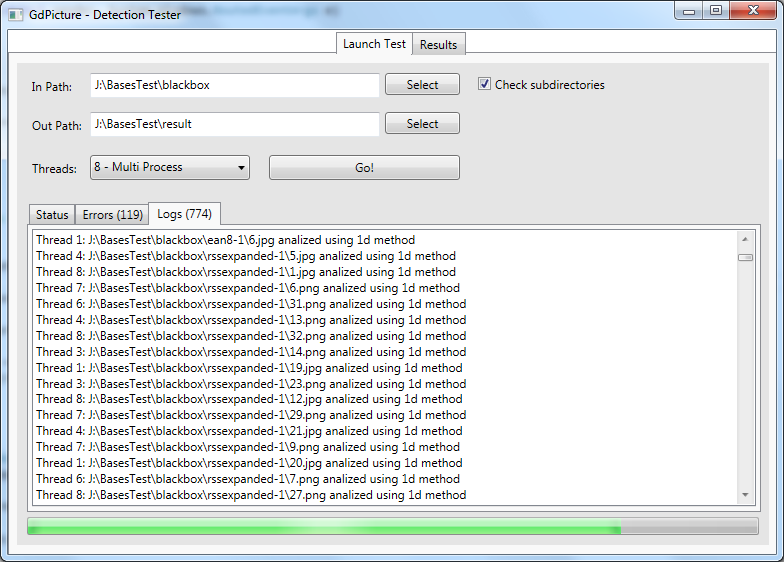
\includegraphics[scale=0.5]{images/projet1DetectionWindow.png}
\end{center}
\caption{Une détection en cours}
\end{figure}

\subsection{Création de rapports}

Chaque passage sur la base de tests va générer un rapport. L'un des objectifs de l'application est de pouvoir comparer plusieurs rapports. Le cas typique d'utilisation sera la réalisation d'un nouveau rapport à chaque nouvelle version du moteur de détection. Il est donc important de pouvoir stocker ces rapports afin de pouvoir les comparer au moment voulu. Le meilleur moyen est d'utiliser des fichiers.

Pour pouvoir structurer l'information dans un fichier, il faut utiliser une norme de notation. C'est à ça que servent les langages comme XML et ses dérivés. J'avais dans un premier temps commencé à utiliser XML mais très vite j'ai été limité par les contraintes de mise en forme du langage. Je me suis donc tourné vers un format plus récent : JSON. Historiquement dédié au web, JSON a l'avantage de disposer d'une syntaxe simple et souple.

J'ai pu trouver une bibliothèque .NET gérant la traduction en JSON\footnote{Disponible ici : http://james.newtonking.com/projects/json-net.aspx}. L'intérêt de cette bibliothèque est qu'elle permet de faire abstraction de la constitution d'un objet pour le traduire\footnote{On dit de cet objet qu'il est \og parsé \fg{} }. Il me suffit de donner un objet à une fonction de parsage pour qu'elle me renvoie le résultat en JSON. Il ne me reste donc qu'à écrire ce résultat dans le fichier.

En appliquant cette opération à toutes les images, on obtient donc un fichier contenant l'ensemble des informations de la détection pour toute la base de tests.

\subsection{Présentation des résultats}

A tout moment, il est possible de comparer les rapports existants. Pour plus de commodité tous les rapports doivent être placés dans le même répertoire. Avec le chemin de ce répertoire, l'application doit être capable de retrouver les informations de chaque rapport et de les classer. Il est ensuite possible de choisir un rapport comme référence et d'afficher les différences de détection dans chaque rapport relativement à celui-ci. On étudie ici le taux de détection, c'est à dire le nombre de codes-barres corrects par rapport au nombre total.

Pour construire l'interface graphique, j'utilise les outils intégrés à Visual Studio. La couche logicielle gérant les graphismes est WPF\footnote{Windows Presentation Foundation, apparue avec la version 3.0 du framework .NET}. Elle permet de gérer la disposition des éléments graphiques et les événements (actions de l'utilisateur). WPF a pour principe de séparer l'interface statique (avant-plan de l'application) avec la gestion dynamique de la fenêtre (arrière-plan) en utilisant deux langages :
\begin{itemize}
\item Le XAML pour l'avant-plan. Il s'agit d'un dérivé de XML qui permet une manipulation aisée des éléments grâce à l'arborescence.
\item Le C\# pour l'arrière-plan. On profite ainsi d'une interface avec le reste de l'application.
\end{itemize}

En pratique, j'ai souvent été amené à utiliser le C\# pour manipuler les éléments graphiques, notamment lorsque je devais en générer automatiquement.

Les résultats des différents rapports sont présentés sur quatre niveaux :

\clearpage

Le premier niveau représente les rapports qui ont été détectés dans le répertoire spécifié. Ils sont classés par date et le plus récent est automatiquement défini comme référence. Il est possible de définir un rapport particulier comme référence. On affiche quelques informations propres à chaque rapport comme la date, l'heure, la version de GdPicture et le nombre de fichiers.

\begin{figure}
\begin{center}
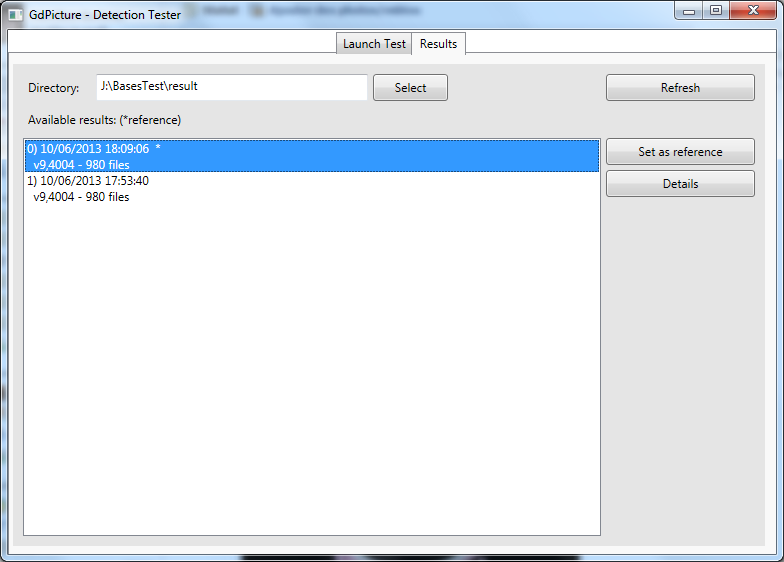
\includegraphics[scale=0.5]{images/projet1RapportWindow.png}...
\end{center}
\caption{La liste des rapports détectés}
\label{niveau1}
\end{figure}

\clearpage

Le second niveau de résultats présente les différences de taux de détection entre la référence et les autres rapports. Ces différences sont détaillées pour chaque type de détection. C'est à ce stade que l'on se rend compte le mieux des problèmes de détection qui peuvent survenir comme ceux expliqués plus haut.

\begin{figure}
\begin{center}
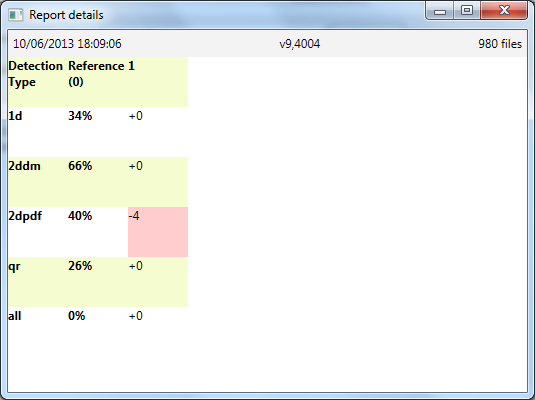
\includegraphics[scale=0.6]{images/projet1RapportWindow2.png}
\end{center}
\caption{Comparaison des taux de détection entre les rapports}
\label{niveau2}
\end{figure}

\clearpage

Le troisième niveau présente l'état de détection de chaque fichier d'un rapport pour le type de détection donné. Le niveau précédent propose des zones cliquables, on peut donc choisir d'afficher les détails pour un rapport (en colonne) et un type de détection (en ligne). Cela permet de rechercher quel fichier a pu causer les différences de détection constatées au niveau 2.

Trois cas sont possibles :
\begin{description}
\item[OK :] Le code-barres a été détecté et est correct
\item[Undetected :] Aucun code-barres n'a été détecté
\item[Incorrect :] Un code-barres a été détecté mais il ne correspond pas à la valeur de contrôle.
\end{description}

\begin{figure}
\begin{center}
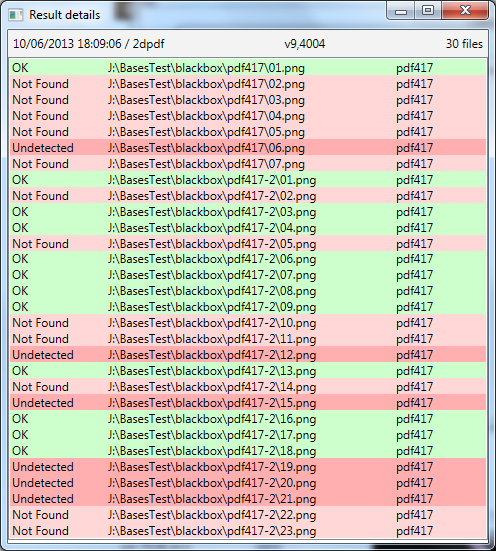
\includegraphics[scale=0.6]{images/projet1RapportWindow3.png}
\end{center}
\caption{Etat de détection détaillé par fichier}
\label{niveau3}
\end{figure}

Il est possible de double-cliquer sur une ligne pour accéder à l'historique du fichier : c'est le quatrième niveau.

\clearpage

Le quatrième niveau présente un historique de détection du fichier image sur les différents rapports. Il détaille le nombre de codes-barres détectés pour chaque type de détection, le nombre de codes-barres corrects et le statut de détection retourné par GdPicture. Lorsque le statut de détection est différent de \og OK \fg{}, cela est sûrement la cause de variations du taux de détection.

\begin{figure}
\begin{center}
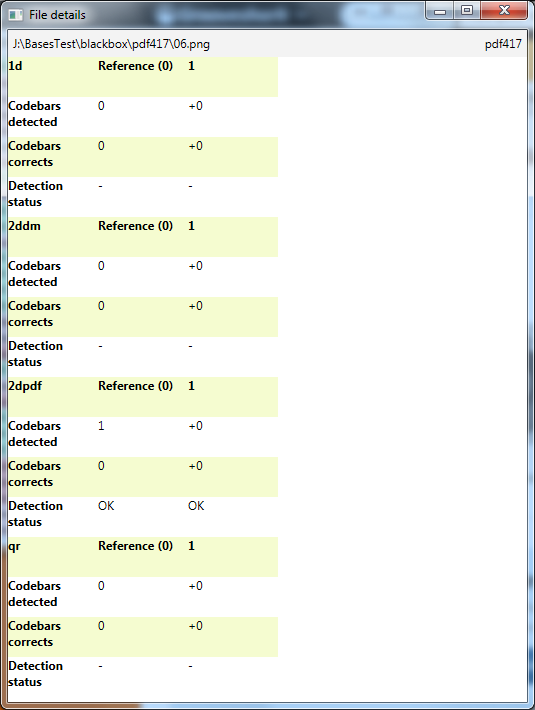
\includegraphics[scale=0.6]{images/projet1RapportWindow4.png}
\end{center}
\caption{Etat de détection détaillé pour un fichier}
\label{niveau4}
\end{figure}

\clearpage
\section{Bilan}

L'enjeu de cette application était de fournir à ORPALIS un moyen de surveiller simplement les différences de détection entre les différentes versions du moteur. Une fois le jeu de test organisé et l'application configurée, il est très rapide de lancer une détection sur la base de test, d'enregistrer le rapport avec ceux existants et de comparer les résultats. La classification par type de détection, puis par fichier permet de donner un maximum d'informations tout en garantissant des résultats organisés et une analyse pertinente.

Ce projet aura été l'occasion de découvrir le langage C\#, l'environnement .NET et la spécification graphique WPF. L'utilisation des outils Microsoft assure la meilleure intégration de l'application dans Windows, permettant ainsi d'obtenir une application performante sans un gaspillage trop important de ressources. Le modèle d'application multithreadée de Loïc m'a permis de faire abstraction de cette contrainte dans la découverte de mon espace de travail. J'ai dû tout de même m'y confronter et construire mon application à l'intérieur. C'est en analysant le code source donné et en y greffant le mien que j'ai pu comprendre le fonctionnement du multi-threading en C\#.

La création de l'interface graphique a pris beaucoup de temps. WPF\footnote{Windows Presentation Foundation} est une technologie 100\% Windows qui nécessite un temps d'adaptation. Ma principale difficulté a été de construire des interfaces complexes dans la présentation des résultats, notemment au niveau 2.

L'utilisation des ressources a été un point central d'optimisation. N'étant pas familier avec les outils Microsoft, j'ai dû m'adapter à des techniques de programmation qui m'étaient étrangères. Je dois avouer que je n'avais jamais eu à m'intéresser à la quantité de ressources qu'utilisait mon application, alors qu'il s'agit d'une préoccupation importante.

Le point positif est que j'ai pu profiter d'une part de l'expérience de Loïc et Cédric, d'autre part de la grande quantité d'informations disponibles sur les sites de Microsoft, les forums et autres communautés de développeurs .NET.
\chapter{Un lecteur virtuel de codes-barres}

Après que l'application de test ait été achevée, je me retrouvai sans activité alors qu'il me restait la moitié de mon stage.
C'est ainsi que je me lançai dans un projet de détecteur virtuel de codes-barres.
Me basant sur le moteur de détection de GdPicture que je connaissais désormais, j'ai développé une application ergonomique et simple qui simule un lecteur de codes-barres sur des images ou des documents scannés.

\section{Objectifs}

Cette application devait tout d'abord reproduire le fonctionnement des lecteurs de codes-barres filaires existants.
Il devait être possible d'accéder rapidement à l'application depuis n'importe quelle autre, et que le lecteur soit une extension de la souris.
Enfin, plusieurs actions devaient être possibles une fois un code-barres détecté :
\begin{itemize}
\item Copier le résultat dans le presse-papier
\item Envoyer le résultat vers une autre fenêtre pour qu'elle le traite comme une entrée clavier
\end{itemize}

\section{Développement}

J'ai choisi de créer une application sans fenêtre, c'est à dire qui s'exécuterait d'une manière transparente pour l'utilisateur, et accessible depuis la zone de notifications\footnote{En anglais : \og system tray \fg{} ou plus simplement \og systray \fg{}}.
J'ai pour cela utilisé une bibliothèque WPF\footnote{Disponible ici : http://www.hardcodet.net/projects/wpf-notifyicon} prenant en charge cette fonctionnalité. Il m'est alors possible de créer une icône dans le systray, de créer un menu pour le clic-droit, de gérer les événements de clic et les info-bulles.

On peut voir dans la figure \ref{systrayMenu} le menu de l'application :
\begin{itemize}
\item Une case à cocher pour copier automatiquement le résultat d'une détection dans le presse-papiers
\item Una case à cocher pour l'envoyer dans une fenêtre.
\item Une liste pour choisir ladite fenêtre
\item Un bouton \og Plus d'options \fg{} qui ouvre une fenêtre permettant de choisir les types de codes-barres que l'on souhaite détecter.
\end{itemize}

\begin{figure}
\begin{center}
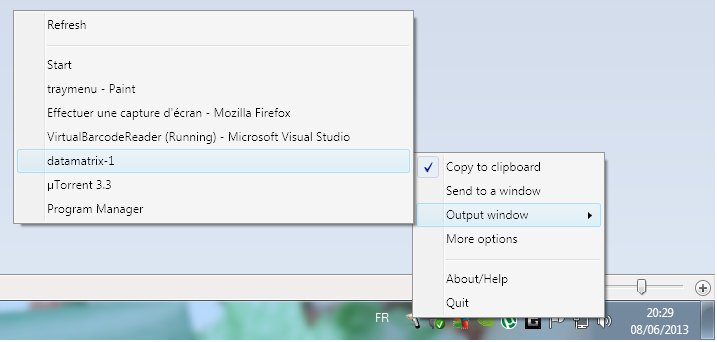
\includegraphics[scale=0.7]{images/traymenu.png}
\end{center}
\caption{Le lecteur de code-barres dans le systray}
\label{systrayMenu}
\end{figure}

\subsection{Envoyer des caractères à une autre application}

Une fonctionnalité intéressante du lecteur virtuel est de pouvoir définir une application vers laquelle seront redirigés les résultats des détections. Cela permet par exemple de remplir rapidement des formulaires en limitant le nombre de clics. Dans ce cas, je fais en sorte que le résultat soit envoyé à la fenêtre comme s'il avait été tapé au clavier.

On commence par récupérer un identifiant unique, appelé \og handle \fg{} associé à la fenêtre voulue :

\verb|int iHandle = NativeWin32.FindWindow(null, selectedWindow);|

Cette fonction est un portage d'une fonction bas niveau. Pour plus de détails concernant le portage de fonctions Win32, voir l'annexe \ref{hook}. Le premier paramètre de cette fonction n'est pas utile et doit être passé à \verb|null|. Le second paramètre est le nom de la fenêtre, récupéré plus tôt avec une autre fonction bas niveau listant toutes les fenêtres ouvertes.

On passe la fenêtre au premier plan afin qu'elle soit activée et puisse être prête à recevoir le message :

\verb|NativeWin32.SetForegroundWindow(iHandle);|

Enfin, on envoie le message à l'aide d'une méthode existante dans le framework .NET :

\verb|System.Windows.Forms.SendKeys.SendWait(barcode);|

Ainsi on peut voir apparaître les caractères dans un champ de saisie de la fenêtre, si bien sûr un champ avait été préalablement sélectionné. Le fait amusant est que les caractères apparaissent un à un, comme si quelqu'un les avait tapés très rapidement.

\subsection{Gérer les intéractions pendant la détection}

Comme vous pouvez le constater dans la figure \ref{detectionRing}, le double-clic sur l'icône lance la détection matérialisée par un cercle. Pour détailler, il s'agit en fait d'une fenêtre dépouillée de son interface habituelle, dont le fond est transparent et dans laquelle une ellipse est dessinée.

\begin{figure}
\begin{center}
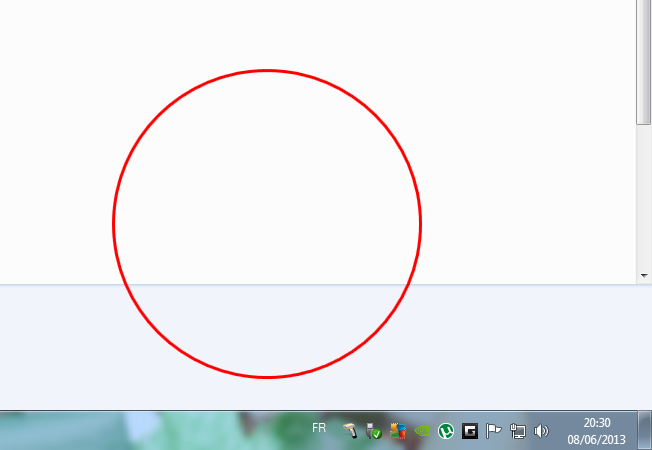
\includegraphics[scale=0.5]{images/detector.png}
\end{center}
\caption{Détection en cours}
\label{detectionRing}
\end{figure}

Grâce à des mécanismes avancés décrits dans l'annexe \ref{hook}, je peux récupérer certains événements utilisateurs comme le mouvement de la souris qui va provoquer le déplacement de la fenêtre de sorte que le curseur reste toujours au centre du cercle. Je vais aussi intercepter des événements plus complexes comme l'appui simultané des touches CTRL et MAJ et de la rotation de la molette de la souris. Cette action va permettre de faire varier la taille du cercle et donc la surface de détection. Je vais enfin intercepter tous les clics afin de m'assurer que le cercle reste en permanence au premier plan, sans quoi il serait vite perdu de vue derrière les autres fenêtres, sans possibilité de le ramener à l'avant-plan car la fenêtre ne possède pas d'icône dans la barre de tâche.

Le principe de la détection est de lancer à intervalle régulier une analyse de la zone survolée par le cercle de détection. Cette analyse consiste à capturer la zone de l'écran, à l'enregistrer dans une image en mémoire et à soumettre cette image à GdPicture en suivant le même principe que dans le premier projet que j'ai réalisé. Le choix des fonctions de détection à utiliser se fait cette fois-ci à l'aide des informations saisies par l'utilisateur dans la section \og Plus d'options \fg{}. En plus de la valeur du code-barres, je récupère son type afin de filtrer, toujours suivant les mêmes paramètres\footnote{En plus des types de détection habituels (DataMatrix, QRcode, etc.), il existe plusieurs familles de codes-barres 1D qui sont connues de GdPicture et qui peuvent être filtrées}.

Une fois qu'un code-barres est détecté, les actions automatiques se lancent si elles ont été activées. Il est toutefois possibles de les lancer manuellement :
\begin{itemize}
\item CTRL + MAJ + S pour envoyer le résultat à une fenêtre
\item CTRL + MAJ + D pour afficher une info-bulle contenant la valeur du code-barres
\item CTRL + MAJ + C pour copier le résultat dans le presse-papiers
\end{itemize}

\begin{figure}
\begin{center}
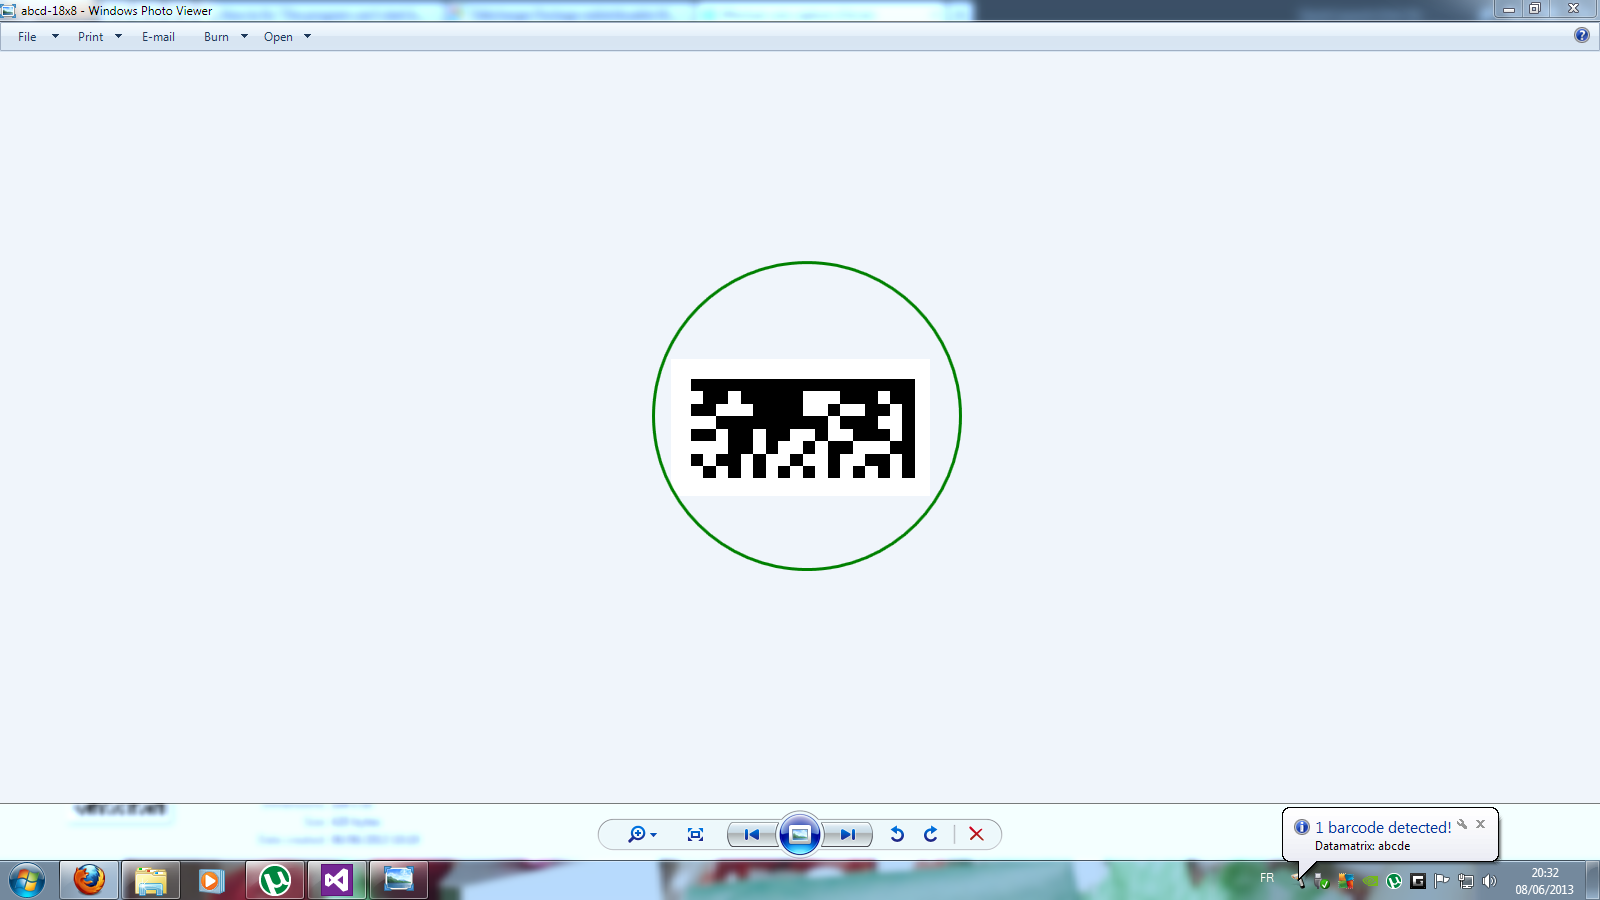
\includegraphics[scale=0.3]{images/detected.png}
\end{center}
\caption{1 code-barres détecté}
\label{detectedBarcode}
\end{figure}

\clearpage

\section{Bilan}

Ce second projet a été pour moi l'occasion d'approfondir mes connaissances dans les technologies que j'avais découvertes lors de mon premier projet. J'ai pu en effet mesurer mes progrès en relisant les premières lignes que j'avais écrites au début de mon stage, certaines me laissant dubitatif quant à leur qualité.

La réalisation de cette application m'a également permis de sortir du sujet initial de mon stage. J'ai pu me concentrer sur un sujet très différent, mais tout aussi intéressant. Malgré les longs moments passés à rechercher de la documentation sur certains mécanismes complexes, je garde le souvenir d'une application que je me suis amusé à créer.

Enfin, le lecteur de codes-barres virtuel est à destination du grand public, contrairement à l'application de tests. J'ai apprécié la volonté d'ORPALIS de supporter ce projet en le distribuant sur son site web sous le nom \og ORPALIS Virtual Barcode Reader \fg{} tout en laissant mon nom sur le produit.


\chapter*{Conclusion}
\chapter*{Glossaire}

\appendix
\titleformat{\chapter}[display]{\sf\bfseries\Huge} {\vspace{-10ex} \large\MakeUppercase{Annexe}~\large\thechapter} {2ex}{\titlerule\vspace{1ex}\filright}
\part*{Annexes à l'application de tests de non-régression}
\chapter{Comment organiser la base de tests et configurer l'application ?}
\label{configFile}
La configuration de l'application dépend grandement de l'architecture de la base de tests.













\chapter{Comment un fichier est-il traité par l'application ?}

Afin de pouvoir analyser les informations contenues dans l'intégralité du jeu de test, il est nécessaire au préalable d'organiser ces informations. Plusieurs structures sont présentes pour assurer un agencement clair, et une traduction simple des données. Afin de décrire comment chacune entre en jeu, nous allons détailler un exemple de test.

\section{Détection}

\subsection{Principe}

Notre jeu de test est constitué d'un nombre \verb|n| d'images. Chaque image peut contenir un ou plusieurs codes-barres. Le processus de détection s'effectue dans la classe \verb|Model|. Lors de l'analyse d'une image, \verb|Model| crée un objet \verb|Barcode| par code-barres détecté, et le met dans un objet \verb|FileResult| qui correspond donc au résultat d'une détection pour un fichier.

\begin{figure}
\begin{center}
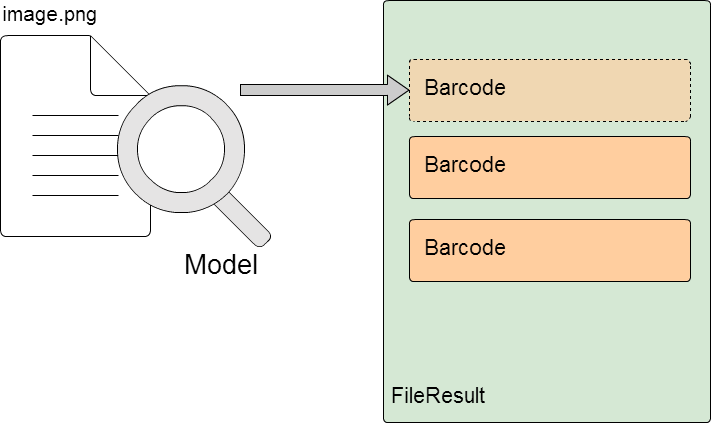
\includegraphics[scale=0.3]{images/projet1Detection.png}
\caption{Le processus d'analyse d'une image}
\end{center}
\end{figure}

Un objet \verb|Barcode| contient :
\begin{itemize}
\item La valeur du code-barres
\item Une valeur booléenne indiquant si le code-barres est correct au regard du fichier témoin de l'image
\item Le type du code-barres (1D, QRcode, etc.)
\end{itemize}

Un objet \verb|FileResult| contient bien sûr une liste de \verb|Barcode|, mais aussi :
\begin{itemize}
\item Le nom de l'image
\item Le nom du fichier témoin qui lui est associé
\item La catégorie, c'est à dire la valeur qui représente le répertoire de l'image dans le fichier de configuration
\item Le type de détection tel que spécifié dans le fichier de configuration
\item La liste des valeurs de controle contenues dans le fichier témoin
\item Un dictionnaire présentant l'état de la détection pour chaque type de codes-barres.
\end{itemize}

\subsection{Explication de code}

La classe \verb|Model| contient une méthode servant à la détection d'une image :\\\verb| DetectionError detectBarCode(string _nomFic, out FileResult file);|

Cette fonction prend en paramètre d'entrée le chemin de l'image. En paramètre de sortie, un objet de type \verb|FileResult| qui représente le résultat de la détection pour cette image. Cette fonction retourne une valeur de type \verb|DetectionError| qui est en fait une énumération à trois valeurs :
\begin{description}
\item[OK :] aucun problème détecté.
\item[CONTROL\_VALUE\_ERROR :] valeur de contrôle introuvable (lorsque le fichier témoin de l'image est introuvable ou mal nommé).
\item[DETECTION\_TYPE\_ERROR :] lorsque le répertoire de l'image n'est pas référencé dans le fichier de configuration.
\end{description}

Voici donc le contenu de cette fonction :
\newpage
\begin{lstlisting}
public DetectionError detectBarCode(string _nomFic, out FileResult file)
{
  file = new FileResult(_nomFic);
  file.CodeType = getCategory(file.Filename);
  file.DetectionType = getDetectionType(file.CodeType);

  // Checks if the detection type is correct
  if (file.DetectionType == String.Empty)
  {
    return DetectionError.DETECTION_TYPE_ERROR;
  }
  // Checks if the file test exists
  else if (!File.Exists(file.FilenameControl))
  {
    return DetectionError.CONTROL_VALUE_ERROR;
  }
  else
  {
    int image = this.gpi.CreateGdPictureImageFromFile(_nomFic);
    switch (file.DetectionType)
    {
      case "1d":
        detect1D(image, ref file)
        break;
      case "2ddm":
        detect2DDM(image, ref file);
        break;
      case "2dpdf":
        detect2DPDF(image, ref file);
        break;
      case "qr":
        detectQR(image, ref file);
        break;
      case "all":
        detect1D(image, ref file);
        detect2DDM(image, ref file);
        detect2DPDF(image, ref file);
        detectQR(image, ref file);
        break;
      default:
        break;
    }
    this.gpi.ReleaseGdPictureImage(image);
  }
  return DetectionError.OK;
}
\end{lstlisting}
\newpage

Et le commentaire des lignes importantes :
\begin{itemize}
\item[3-5 :] Création du \verb|FileResult| et initialisation de quelques attributs.
\item[19 :] Chargement du moteur de détection avec l'images à analyser. \verb|this.gpi| est un objet créé dans le constructeur de \verb|Model| et qui gère le dialogue entre l'application et le moteur de GdPicture. Il est détruit à la toute fin du test.
\item[20 :] Teste le type de détection définit dans le fichier de configuration. Il y a deux possibilités :
	\begin{itemize}
	\item Un type a été spécifié, on utilise donc la détection sur ce type.
	\item La valeur \emph{all} a été donnée, on fait donc une détection sur tous les types de codes-barres.
	\end{itemize}
\item[43 :] L'image est libérée en mémoire, on est prêt à passer à l'image suivante.
\end{itemize}

\paragraph{}

On remarque l'utilisation de la fonction \verb|detect*(image, ref file)|. En effet, suivant le type de détection, les fonctions de GdPicture à utiliser diffèrent. Voici un exemple avec la détection 1D :

\begin{lstlisting}
private FileResult detect1D(int image, ref FileResult file)
{
  this.gpi.Barcode1DReaderClear();
  Barcode result;
  file.DetectionStatus.Add("1d", this.gpi.Barcode1DReaderDoScan(image).ToString());
  int nbDetected = this.gpi.Barcode1DReaderGetBarcodeCount();
  for (int i = 0; i < nbDetected; i++)
  {
    result = new Barcode();
    result.barcode = gpi.Barcode1DReaderGetBarcodeValue(i + 1).Trim();
    result.detected = file.ControlBarcodes.Contains(result.barcode);
    result.detectionType = "1d";
    file.Barcodes.Add(result);
  }
  return file;
}
\end{lstlisting}

\begin{itemize}
\item[3 :] Nettoyage des éventuels précédentes détections
\item[5 :] Ajout de l'état de la détection renvoyé par la fonction de scan de GdPicture
\item[6 :] Récupération du nombre de codes-barres détectés
\item[7 :] Pour chaque code-barres, création d'un objet \verb|Barcode|, récupération de sa valeur et comparaison avec le fichier témoin. Ajout du code-barre au \verb|FileResult|.
\end{itemize}

On peut donc voir ici comment les codes-barres sont détectés et comment les résultats sont stockés dans des objets. Intéressons-nous maintenant à la création de rapports.

\section{Création de rapports}

La création de rapports s'effectue au sein de la classe Report. Son travail est de rassembler les résultats de tous les fichiers de la base de tests (contenus dans des \verb|FileResult|). Pour cela, elle crée un objet \verb|ReaderReport| qui représente un rapport, c'est à dire une analyse complète de la base de tests. En plus des informations de chaque fichier, elle contient des informations propres au rapport dans un objet \verb|ExtraReportInfo|. Elle parse ensuite le \verb|ReaderReport| dans un fichier JSON pour qu'il puisse être réutilisé.

\begin{figure}
\begin{center}
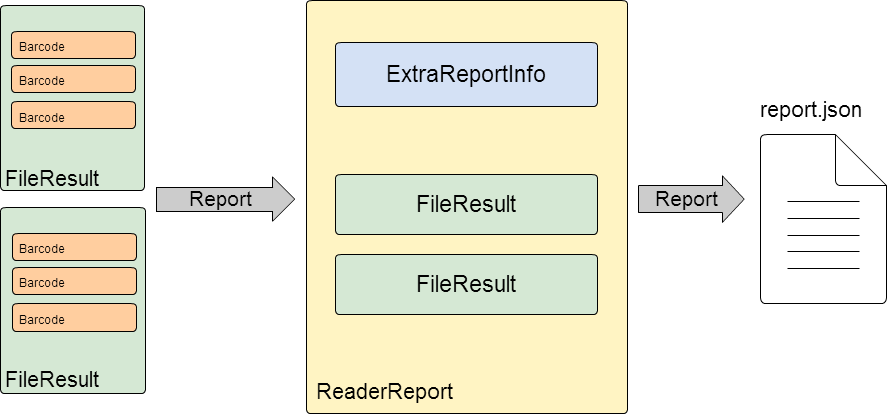
\includegraphics[scale=0.5]{images/projet1Rapport.png}
\caption{Le processus de création de rapport}
\end{center}
\end{figure}

Un objet \verb|ExtraReportInfo| contient plusieurs informations propres au rapport :
\begin{itemize}
\item La version courante de GdPicture
\item Une chaine représentant la date et l'heure de la détection
\item Le nombre de fichiers analysés
\item La liste des types de codes-barres connus
\item La liste des catégories (lié au fichier de configuration)
\end{itemize}

\section{Analyse des rapports}



\part*{Annexes au lecteur virtuel de codes-barres}
\chapter{Gestion du clavier et de la souris dans une application non-fenêtrée}
\label{hook}

Cette annexe a pour but de présenter ce qui m'a posé le plus de problèmes lors de la réalisation du lecteur virtuel de codes-barres. La gestion des événements clavier et souris est intégrée à WPF et s'avère très pratique pour intercepter les événements dans une fenêtre. Le problème est tout autre lorsqu'il s'agit d'intercepter des événements hors d'une fenêtre. Dans le cadre de mon application, les événements se déroulent à 90\% hors d'une fenêtre, puisque l'application se lance dans le systray. C'est pourquoi j'ai dû trouver une solution pour pallier à cette carence de WPF.

On peut d'ailleurs expliquer ce manque par une volonté de Microsoft d'empêcher les applications d'intéragir avec le système à un niveau trop bas. En d'autres termes, les applications doivent se tenir à leur place. Cela peut être aussi une contrainte de conception, puisque le système Windows repose sur de vieilles bases datant du début du projet. Ainsi, le seul moyen d'avoir une interactivité complexe avec le système est de faire appel à l'API bas niveau de Windows : Win32.

Le Framework .NET fonctionne en code dit \og managé \fg{}, c'est à dire que le code écrit par le programmeur ne sera pas directement compilé en langage machine, il sera compilé puis interprété par une machine virtuelle qui effectue des vérifications et des optimisations sur le code. Le même concept existe pour le langage Java qui s'exécute à travers la JVM\footnote{Java Virtual Machine}.

L'API Win32 ne fonctionne pas en code managé, et cela pose une limite majeure de conception avec .NET. Toutefois, des outils existent pour appeler des fonctions Win32 dans du code C\#. L'un de ces outils que j'ai pu utiliser est P/Invoke. Il permet d'inclure une DLL système contenant du code non-managé et d'assurer l'interface avec le code managé. Voici un exemple d'utilisation :

[CODE]

Je me suis rendu compte au fil de mes recherches que le seul moyen d'intercepter un événement souris ou clavier à l'extérieur d'une fenêtre était de mettre en place un mécanisme bas niveau appelé \og Hook \fg{}. Un hook (crochet) permet de surveiller les messages transitant des périphériques au système et de les faire bifurquer par l'application. L'application peut surveiller ces messages et soit les laisser passer soit les traiter tout en prenant soin de les relâcher dans leur direction initiale. Comme dit précédemment, le hook est un mécanisme de bas niveau qui se trouve dans une DLL Win32. C'est là que P/Invoke entre en jeu.

Une fois les bonnes fonctions intégrées au projet, il faut traduire les messages qu'elles renvoient par des événements C\#. Enfin, il suffit d'affecter des traitements à ces événements pour obtenir l'intéraction tant espérée. Dans le cadre de mon projet, j'avais effectué ce travail à hauteur de 40\% avant de trouver une bibliothèque C\# basée sur le même principe, mais aussi plus propre et plus complète.

La plus grande difficulté a été de comprendre le fonctionnement du système de hooks. L'intéraction entre l'API bas niveau et le code managé représente un défi majeur de toute application complexe, et est la preuve que sous une apparence simple et conviviale peut se cacher une véritable usine à gaz.

\backmatter
\chapter*{Résumé}
\addcontentsline{toc}{chapter}{Résumé}

Afin de clore mes deux années d'études d'Informatique à l'IUT de Blagnac, j'ai effectué un stage dans une petite entreprise nommée ORPALIS. Ce stage a duré du 8 avril au 14 juin 2013. Le but de ce stage était de réaliser une application de tests de non-régression pour un moteur de détection de codes-barres. Une telle application serait utilisée par l'équipe d'ORPALIS pour avoir des statistiques sur les performances du moteur et d'analyser leur évolution tout au long des nouvelles versions du logiciel. L'environnement de travail était un environnement Microsoft, j'ai donc utilisé le logiciel Visual Studio 2012 ainsi que le langage C\# pour accomplir ma tâche. La compréhension du framework .NET et de l'écosystème centré autour du système d'exploitation Windows m'a permis de créer une application à la fois puissante et simple d'utilisation.

Une fois ce premier projet terminé, j'ai complété mes connaissances en créant une deuxième application tournée cette fois vers le grand public servant à lire des codes-barres. Cette application est conçue pour rendre la détection de codes-barres aussi simple qu'avec un lecteur filaire.

Ces deux projets ont été l'occasion de découvrir le travail au sein d'une petite équipe et m'ont permis d'affiner mon projet professionnel. Je suis prêt à entreprendre des études en école d'ingénieurs afin de développer une expertise dans le génie logiciel.
\chapter*{Abstract}
\addcontentsline{toc}{chapter}{Abstract}

My placement in the ORPALIS company ended my two-years degree in computer science at the University Institute of Technology of Blagnac. It started on the 8\up{th} of April and finished on the 14\up{th} of June 2013. The topic of my placement was to create a regression testing application for a barcode recognition engine developed by the company. The ORPALIS team needed to have a global vision of the engine efficiency by observing the evolution of the recognition rate with the new versions of the software. I worked in a Microsoft environment, that's why i used the Integrated Development Environment Visual Studio 2012 and the C\# language. Understanding the .NET Framework and the Windows Operating System permitted me to develop an efficient easy-to-use software.

Once this project achieved, i completed my knowledge in the .NET development by creating a second application: a virtual barcode reader. This consumer software had to be as simple as the real wired barcode readers.

These two projects allowed me to discover small team working and made me change my professional goals. Indeed, i feel ready to continue studying computer science in engineering school in order to develop my skills in software engineering.

\end{document}